\chapter{LLMalMorph 的详细设计}

\section{A. LLMalMorph 框架}

在本节中,我们将详细阐述我们框架的架构(见图\ref{fig:4.1})。LLMalMorph 分为两个主要模块。第一个模块,功能变异模块使用 LLM 和策略性生成的提示来转换恶意软件源代码函数。第二个模块,变种合成模块将转换后的函数集成回源代码,编译修改后的项目以生成恶意软件变体。该模块还融入了人在回路流程用于编译期间的调试。第一个模块又包含三个关键子模块:Extractor、Prompt Generator 和 LLM Based Function Modifier。第二个模块包含两个主要子模块:Merger 以及 Compilation and Debugging。我们现在介绍支撑该框架的形式化算法,随后对各模块进行详细解释。

\begin{figure}[htb]
	\centering
	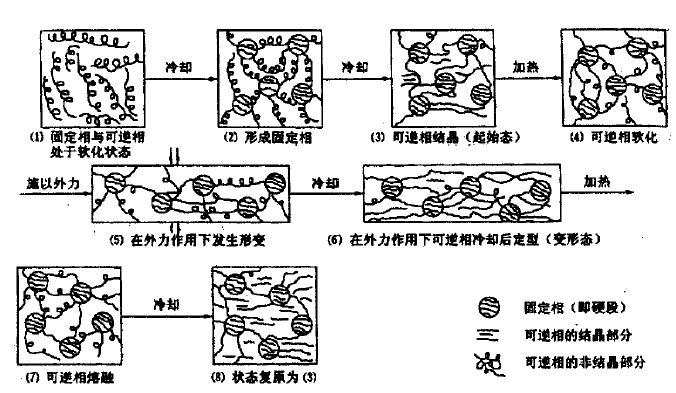
\includegraphics[width=1.15\textwidth]{figures/figure1.png}
	\caption{LLMalMorph整体架构。该框架由两大核心模块构成:功能变异模块:从恶意软件源代码文件中提取功能函数,并借助LLM进行修改。变种合成模块:将修改后的函数更新至恶意软件源代码,通过编译项目生成变种文件}\label{fig:4.1}
\end{figure}

Algorithm \ref{alg:Function Transformation Using LLM},专为功能变异模块设计,详细说明了三个子模块 Extractor、Prompt Generator 和 LLM-Based Function Modifier 如何转换恶意软件源代码中的函数。该算法以文件名 $i$、要修改的函数数量 $j$、期望的转换策略 $s$ 以及选定的 $LLM$ 作为输入。接下来,我们将详细描述每个子模块。

\begin{algorithm}[htbp]
	\caption{使用LLM转换函数\label{alg:Function Transformation Using LLM}}
	\KwIn{文件名$i$,需要改变的函数数量 $j$,转换策略 $s$,语言模型 $LLM$}
	\KwOut{转换后的函数集$\hat{F_{s}}=\{\hat{f_{1}^{i}},\hat{f_{2}^{i}}...,\hat{f_{j}^{i}}\}$}

    Headers,globals,functions$\{f_{1}^{i},f_{2}^{i},...,f_{G}^{i}\}\leftarrow extractor(i)$;\\
    初始化转换后的函数集 $\hat{F_{s}}\leftarrow \emptyset$;\\

    \For{$t \gets 1$ \KwTo $j$}{
        $p_{s}||f_{t}^{i} \leftarrow gen\_prompt(s,f_{t}^{i},headers,globals)$;\\
        Transform function: $\hat{f_{t}^{i}} \leftarrow LLM(p_{s}||f_{t}^{i})$;\\
        Update set: $\hat{F_{s}} \leftarrow \hat{F_{s}} \cup \{\hat{f_{t}^{i}}\}$;
    }
    return $\hat{F_{s}}$
\end{algorithm}

\subsection{Extractor子模块}
Extractor 子模块(算法 \ref{alg:Function Transformation Using LLM} 的第 1 行)利用 extractor 子程序,该子程序接收一个源文件并遍历源代码的解析树。它从解析树中提取并存储以下两条辅助信息:全局声明的变量、结构体、编译器指令的列表,并将它们存储于 $globals$ 中;以及所包含头文件的列表,并将它们存储于 $headers$ 中。此类信息对于成功转换至关重要,因为它提供了函数可能使用的全局依赖项的基本上下文。以提示的形式将此上下文提供给 LLM 可确保生成更准确且语法正确的代码。此后,该子程序解析源文件以提取所有函数定义,生成集合$\{f_{1}^{i},f_{2}^{i},...,f_{G}^{i}\}$。

\subsection{Prompt Generator子模块}
算法 \ref{alg:Function Transformation Using LLM} 的第 3−7 行对应于 Prompt Generator 和 LLM Transformation 子模块。第 4 行中的子程序 $gen\_prompt$ 被调用,参数为函数 $f_t^{i}$、转换策略 $s$ 以及提取的 $headers$ 和 $globals$。它将输入代码和策略构造成一个为 LLM 定制的提示 $p_{s}||f_{t}^{i}$。提示的设计详见第 IV-C 节。另请参阅附录 F 了解该子程序中使用的不同类型的提示,以及附录 G 了解一个完整构建的提示及其相应 LLM 响应的示例。

\subsection{LLM Based Function Modifier子模块}
算法 \ref{alg:Function Transformation Using LLM}的第5行将设计好的提示 $p_{s}||f_{t}^{i}$ 提供给选定的$LLM$,并获取转换后的函数。在代码生成过程中,我们使用了LLM的默认推理设置。具体而言,temperature=0.8,top-k=40,top-p=0.9。我们在附录A-A中提供了使用LLM进行代码生成过程的详细描述。

最后,第 6 行将转换后的函数 $f_{t}^{i}$ 追加到输出集合中。一旦所有选定的函数处理完毕,该算法即返回转换后的集合。我们注意到,该算法可以执行多次,以从同一源文件生成函数的多个变体。然而,在本工作中,对于每个选定的恶意软件样本,我们将评估限制在转换后函数的单一版本上。

Algorithm \ref{alg:Malware Variant Generation},在变种合成模块中实现,使用由算法 \ref{alg:Function Transformation Using LLM} 产生的转换后函数集合 $\hat{F_{s}}$、恶意软件项目 $P$ 以及被修改的文件 $i$。它以增量方式生成恶意软件变体,并结合手动调试以确保成功编译。第 1 行初始化恶意软件变体的结果集合 $M_{s}$。该集合包含针对文件 $i$ 使用策略 $s$ 生成的恶意软件变体。尽管我们展示了针对某个特定文件的算法,但当我们处理后续文件时,先前处理过的文件的所有修改都会被保留并向前传递,从而确保恶意软件代码库的累积式转换。该算法的核心功能封装在第 2-10 行中,其中每个转换后的函数被迭代地集成和调试。

\begin{algorithm}[htbp]
	\caption{恶意软件变种生成\label{alg:Malware Variant Generation}}
	\KwIn{恶意软件项目$P$,文件名 $i$,转换后的函数集合 $\{\hat{f_{1}^{i}},\hat{f_{2}^{i}}...,\hat{f_{j}^{i}}\}$}
	\KwOut{编译后的恶意软件变种集合$M_{s}$}
    初始化集合: $M_s \leftarrow \emptyset$;\\
    \For{$t \gets 1$ \KwTo $j$}{
        Extract subset of functions: $\hat{F_{t}} \leftarrow \{\hat{f_{k}^{i}} \in \hat{F_{s}} | 1\leq k\leq t\}$;\\   
        Generate updated file: $\hat{i} \leftarrow merger(i,\hat{F_{t}})$;\\
        \While{$compile(P)$ fails}{
            Debug project $P$ and resolve errors;
        }
        Compile project: $\hat{M_{s}} \leftarrow compile(P)$;\\
        Add compiled malware: $M_{s} \leftarrow M_{s} \cup \hat{M_{s}}$;\\
    }
    return $M_{s}$
\end{algorithm}

\subsection{Merger子模块}
第 3 行首先提取函数子集 $\hat{F_{t}}$,该子集包含函数 1 到 $t$。下一行使用 $merger$ 子程序,用集合 $\hat{F_{t}}$ 更新文件 i。它将更新后的函数集成到文件 $i$ 中,同时保持其余函数不变,并利用在 LLM 使用算法 \ref{alg:Function Transformation Using LLM} 进行代码生成过程中的各种簿记信息。合并后,我们获得包含 $(1...t)$ 个修改后函数的更新文件 $\hat{i}$。$merger$ 子程序的更多细节详见附录 A-B。

\subsection{Compilation and Debugging子模块}
算法 2 的下一步涉及将更新后的文件 $\hat{i}$ 放入恶意软件项目 $P$ 中。第 6–9 行编译更新后的恶意软件项目。如果编译成功,则将生成的恶意软件变体 $\hat{M_{s}}$ 添加到结果集 $M_{s}$ 中。如果编译失败,则进行手动调试以解决错误。

手动调试由一位从事对抗性恶意软件领域和恶意软件分类研究的研究人员执行,这确保了修正的一致性和技术可靠性。调试过程严格解决语法错误、构建和项目配置问题,例如链接外部库或更改语言版本,以及恢复 LLM 遗留的不完整的占位符代码。未对 LLM 生成代码的语义逻辑进行任何更改。代码修正在成功编译修改后的恶意软件源代码的前提下,被刻意限制在最小干预范围内。值得注意的是,调试过程专注于第 $t$ 个函数,因为先前 $(1,...,t − 1)$ 的 LLM 生成函数已经过调试和修正,确保错误不会跨迭代传播。调试完成后,编译成功的恶意软件变体可执行文件被添加到 $M_{s}$ 中。该过程持续增量进行,直到所有函数处理完毕并返回最终的恶意软件变体集合。

\section{B. 代码转换策略}
我们介绍用于通过LLM操作C/C++恶意软件源代码的源代码转换策略。

\subsection{代码优化}
该策略通过提示优化源代码,方法是消除冗余、解决性能瓶颈以及简化代码逻辑,而不改变其核心功能。它涉及使用替代的数据结构和算法,或利用现代库和特定语言特性,例如C++算法头文件中的搜索函数。这些优化可能改变代码的执行和性能特征,有可能降低静态或基于启发式方法的检测率。

\subsection{代码质量与可靠性}
该策略确保生成的代码遵循标准实践,具有改进的错误处理并解决边缘情况。额外的错误处理可防止执行期间的运行时问题,并为代码添加分支,这使恶意软件更加可靠。

\subsection{代码可重用性}
该策略侧重于将大型函数拆分为更小的模块化块。这些较小的函数调用通过改变执行流,有助于掩盖恶意软件的真实行为,这使得依赖涉及控制流执行模式的检测器在实现恶意软件预期相同结果的同时面临更大挑战。

\subsection{代码安全性}
该策略通过遵循安全编码标准来解决潜在的安全漏洞。恶意软件(如勒索软件)严重依赖加密库进行数据加密和解密。此方法提示 LLM 用替代方案替换这些库,修改敏感操作的实现,同时保持恶意软件的核心功能。通过混淆加密行为,检测引擎可能更难以识别该可执行文件为恶意软件。

\subsection{代码混淆}
该策略通过使代码更难以分析和逆向工程来增强恶意软件的规避能力。它包括用无意义的名称重命名函数和变量、添加不必要的控制流结构(例如,跳转、循环)、改变现有控制流以及插入反调试技术。它还定义并调用多余函数,并添加仅在罕见条件下触发的执行路径。这些转换旨在使静态和动态分析复杂化,同时保留恶意软件的核心功能。

\subsection{Windows API 特定转换}
该策略使用提示来识别恶意软件函数内的 Windows API 调用,并引导 LLM 用替代或间接等效的 API 替换它们。它还可能引入包装函数以模糊直接的 API 使用。我们不是使用静态映射,而是利用 LLM 的生成能力来产生多样化的 API 替换,从而增加变异性并避免预定义映射的僵化性和可扩展性问题。尽管功能保持不变,但改变后的 API 模式可能会混淆基于启发式的检测系统(这些系统通常依赖常见的 Windows API 使用模式),从而使恶意软件更难以检测。

\section{C. LLM的快速设计}
在本节中,我们描述用于生成提示的Algorithm \ref{alg:Prompt Construction Subroutine for LLM-based Function Transformation}。我们还介绍了LLM在转换给定函数$f_{t}^{i}$时必须遵循的约束。

它基于给定的转换策略$s$、第$t$个函数$f_{t}^{i}$以及文件$i$的$headers$和$globals$(如算法\ref{alg:Function Transformation Using LLM}中所定义)进行操作。该子程序以调用$system\_prompt$开始,生成$p_{sys}$。这定义了LLM作为专业编码助手的角色,该助手在系统编程以及C、C++和C\#等语言方面拥有专业知识,并确保代码转换是在适当的上下文和能力范围内进行的。随后,$intro\_prompt$通过接收目标函数$f_{t}^{i}$的名称生成$p_{intro}$,并指定必须使用以下预定义策略将提供的函数以及必要的头文件和全局变量转换为变体函数。接下来,使用$strategy\_prompt$和$s$生成转换策略提示$p_{strat}$。这些步骤建立了转换上下文并指导LLM执行所需的修改。

\begin{algorithm}[htbp]
	\caption{基于LLM实现函数转换的快速构造子程序\label{alg:Prompt Construction Subroutine for LLM-based Function Transformation}}
    \SetKwFunction{FFunOne}{$GEN\_PROMPT$}
    \SetKwProg{Fn}{Function}{:}{end}
    \Fn{\FFunOne{$s$, $f_{t}^{i}$, $headers$, $globals$}}{
        $p_{sys} \leftarrow system\_prompt()$;\\
        $p_{intro} \leftarrow intro\_prompt(f_{t}^{i}.name)$;\\
        $p_{strat} \leftarrow strategy\_prompt(s)$;\\
        $p_{pres} \leftarrow preserve\_rules\_prompt(f_{t}^{i}.name)$;\\
        $p_{addit} \leftarrow additional\_prompt(f_{t}^{i}.name)$;\\
        $p_{code} \leftarrow headers \oplus globals \oplus f_{t}^{i}$;\\
        $p_{user} \leftarrow p_{intro} \oplus p_{strat} \oplus p_{preserve} \oplus p_{additional} \oplus p_{code}$;\\
        return $p_{s}||f_{t}^{i} = p_{sys} \oplus p_{user}$;\\
    }
\end{algorithm}

保留提示$p_{pres}$试图确保原始函数和转换后的函数在语义上等价。它明确指示模型不要修改全局定义或自定义元素(变量、对象、常量)以保持功能一致性,从而避免整个代码库中可能出现的语法或语义错误。此外,$p_{addit}$施加严格的准则以保持一致的、符合语法的代码格式并保留函数签名,指示模型仅在单个特定语言的代码块中生成修改后的函数和必要的头文件,以便于解析和后处理。这确保了输出是完整的,不遗留未完成的代码块,并避免重新生成原始函数。

在完成这些步骤后,代码的提示通过组合 $headers$、$globals$ 和函数 $f_{t}^{i}$ 的定义来构建,其中符号$\oplus$代表字符串连接。这使我们能够通过连接第 3−7 行的所有提示来构建总的用户提示 $p_{user}$。然后,通过连接 $p_{sys}$ 和 $p_{user}$ 来构建最终提示 $p_{s}||f_{t}^{i}$。这种结构化的方法确保 LLM 接收到用于转换任务的明确且完整的指令,同时满足所有必要的约束和要求。

\begin{table}[htbp]
	\centering
	\caption{选择的恶意软件样本总结}
	\label{tab:4.1}
	\begin{tabular*}{\textwidth}{@{\extracolsep{\fill}}cccccccc}
		\toprule
		样本 & 语言 & LOC & 文件数量 & 函数数量 & VT率 & HA率 & 类型 \\
		\midrule
		Exeinfector & C++ & 230 & 1 & 4 & 72.009 & 26.67 & 感染型病毒 \\
		Fungus & C++ & 2266 & 15 & 46 & 73.630 & 76 & 通用犯罪软件 \\
		Dexter & C & 2661 & 12 & 61 & 83.020 & 88 & POS木马 \\
		HiddenVNC & C++ & 4959 & 18 & 60 & 76.503 & 75 & HVNC机器人 \\
		Predator & C++ & 4145 & 10 & 102 & 58.797 & 70.333 & 信息窃取 \\
		Prosto-Stealer & C++ & 7436 & 27 & 143 & 62.033 & 72.333 & 信息窃取 \\
        Conti(Cryptor) & C++ & 8031 & 35 & 99 & 65.275 & 79.333 & 勒索软件 \\
        Babuk(Cryptor) & C++ & 3910 & 22 & 62 & 71.759 & 83.667 & 勒索软件 \\
        RedPetya & C++ & 1494 & 5 & 15 & 62.500 & 56.333 & 勒索软件 \\
        RansomWar & C & 1357 & 5 & 13 & 65.728 & 50.333 & 勒索软件 \\
		\bottomrule
	\end{tabular*}
\end{table}